
\documentclass[letterpaper,hide notes,xcolor={table,svgnames},pdftex,10pt]{beamer}
\def\showexamples{t}


%\usepackage[svgnames]{xcolor}

%% Demo talk
%\documentclass[letterpaper,notes=show]{beamer}

\usecolortheme{crane}
\setbeamertemplate{navigation symbols}{}

\usetheme{MyPittsburgh}
%\usetheme{Frankfurt}

%\usepackage{tipa}

\usepackage{hyperref}
\usepackage{graphicx,xspace}
\usepackage[normalem]{ulem}
\usepackage{multicol}
\usepackage{amsmath,amssymb,amsthm,graphicx,xspace}
\newcommand\SF[1]{$\bigstar$\footnote{SF: #1}}

\usepackage[default]{sourcesanspro}
\usepackage[T1]{fontenc}
\usepackage[scaled]{beramono}
\usepackage{tikzpagenodes}

\newcounter{tmpnumSlide}
\newcounter{tmpnumNote}


% old question code
%\newcommand\question[1]{{$\bigstar$ \small \onlySlide{2}{#1}}}
% \newcommand\nquestion[1]{\ifdefined \presentationonly \textcircled{?} \fi \note{\par{\Large \textbf{?}} #1}}
% \newcommand\nanswer[1]{\note{\par{\Large \textbf{A}} #1}}


 \newcommand\mnote[1]{%
   \addtocounter{tmpnumSlide}{1}
   \ifdefined\showcues {~\tiny\fbox{\arabic{tmpnumSlide}}}\fi
   \note{\setlength{\parskip}{1ex}\addtocounter{tmpnumNote}{1}\textbf{\Large \arabic{tmpnumNote}:} {#1\par}}}

\newcommand\mmnote[1]{\note{\setlength{\parskip}{1ex}#1\par}}

%\newcommand\mnote[2][]{\ifdefined\handoutwithnotes {~\tiny\fbox{#1}}\fi
% \note{\setlength{\parskip}{1ex}\textbf{\Large #1:} #2\par}}

%\newcommand\mnote[2][]{{\tiny\fbox{#1}} \note{\setlength{\parskip}{1ex}\textbf{\Large #1:} #2\par}}

\newcommand\mquestion[2]{{~\color{red}\fbox{?}}\note{\setlength{\parskip}{1ex}\par{\Large \textbf{?}} #1} \note{\setlength{\parskip}{1ex}\par{\Large \textbf{A}} #2\par}\ifdefined \presentationonly \pause \fi}

\newcommand\blackboard[1]{%
\ifdefined   \showblackboard
  {#1}
  \else {\begin{center} \fbox{\colorbox{blue!30}{%
         \begin{minipage}{.95\linewidth}%
           \hspace{\stretch{1}} Some space intentionally left blank; done at the blackboard.%
         \end{minipage}}}\end{center}}%
         \fi%
}



%\newcommand\q{\tikz \node[thick,color=black,shape=circle]{?};}
%\newcommand\q{\ifdefined \presentationonly \textcircled{?} \fi}

\usepackage{listings}
\lstset{basicstyle=\footnotesize\ttfamily,
	breaklines=true,
	aboveskip=15pt,
  	belowskip=15pt,
	frame=lines,
	numbers=left, basicstyle=\scriptsize, numberstyle=\tiny, stepnumber=0, numbersep=2pt
}

\usepackage{siunitx}
\newcommand\sius[1]{\num[group-separator = {,}]{#1}\si{\micro\second}}
\newcommand\sims[1]{\num[group-separator = {,}]{#1}\si{\milli\second}}
\newcommand\sins[1]{\num[group-separator = {,}]{#1}\si{\nano\second}}
\sisetup{group-separator = {,}, group-digits = true}

%% -------------------- tikz --------------------
\usepackage{tikz}
\usetikzlibrary{positioning}
\usetikzlibrary{arrows,backgrounds,automata,decorations.shapes,decorations.pathmorphing,decorations.markings,decorations.text,decorations.pathreplacing}

\tikzstyle{place}=[circle,draw=blue!50,fill=blue!20,thick, inner sep=0pt,minimum size=6mm]
\tikzstyle{transition}=[rectangle,draw=black!50,fill=black!20,thick, inner sep=0pt,minimum size=4mm]

\tikzstyle{block}=[rectangle,draw=black, thick, inner sep=5pt]
\tikzstyle{bullet}=[circle,draw=black, fill=black, thin, inner sep=2pt]

\tikzstyle{pre}=[<-,shorten <=1pt,>=stealth',semithick]
\tikzstyle{post}=[->,shorten >=1pt,>=stealth',semithick]
\tikzstyle{bi}=[<->,shorten >=1pt,shorten <=1pt, >=stealth',semithick]

\tikzstyle{mut}=[-,>=stealth',semithick]

\tikzstyle{treereset}=[dashed,->, shorten >=1pt,>=stealth',thin]

\usepackage{ifmtarg}
\usepackage{xifthen}
\makeatletter
% new counter to now which frame it is within the sequence
\newcounter{multiframecounter}
% initialize buffer for previously used frame title
\gdef\lastframetitle{\textit{undefined}}
% new environment for a multi-frame
\newenvironment{multiframe}[1][]{%
\ifthenelse{\isempty{#1}}{%
% if no frame title was set via optional parameter,
% only increase sequence counter by 1
\addtocounter{multiframecounter}{1}%
}{%
% new frame title has been provided, thus
% reset sequence counter to 1 and buffer frame title for later use
\setcounter{multiframecounter}{1}%
\gdef\lastframetitle{#1}%
}%
% start conventional frame environment and
% automatically set frame title followed by sequence counter
\begin{frame}%
\frametitle{\lastframetitle~{\normalfont(\arabic{multiframecounter})}}%
}{%
\end{frame}%
}
\makeatother

\makeatletter
\newdimen\tu@tmpa%
\newdimen\ydiffl%
\newdimen\xdiffl%
\newcommand\ydiff[2]{%
    \coordinate (tmpnamea) at (#1);%
    \coordinate (tmpnameb) at (#2);%
    \pgfextracty{\tu@tmpa}{\pgfpointanchor{tmpnamea}{center}}%
    \pgfextracty{\ydiffl}{\pgfpointanchor{tmpnameb}{center}}%
    \advance\ydiffl by -\tu@tmpa%
}
\newcommand\xdiff[2]{%
    \coordinate (tmpnamea) at (#1);%
    \coordinate (tmpnameb) at (#2);%
    \pgfextractx{\tu@tmpa}{\pgfpointanchor{tmpnamea}{center}}%
    \pgfextractx{\xdiffl}{\pgfpointanchor{tmpnameb}{center}}%
    \advance\xdiffl by -\tu@tmpa%
}
\makeatother
\newcommand{\copyrightbox}[3][r]{%
\begin{tikzpicture}%
\node[inner sep=0pt,minimum size=2em](ciimage){#2};
\usefont{OT1}{phv}{n}{n}\fontsize{4}{4}\selectfont
\ydiff{ciimage.south}{ciimage.north}
\xdiff{ciimage.west}{ciimage.east}
\ifthenelse{\equal{#1}{r}}{%
\node[inner sep=0pt,right=1ex of ciimage.south east,anchor=north west,rotate=90]%
{\raggedleft\color{black!50}\parbox{\the\ydiffl}{\raggedright{}#3}};%
}{%
\ifthenelse{\equal{#1}{l}}{%
\node[inner sep=0pt,right=1ex of ciimage.south west,anchor=south west,rotate=90]%
{\raggedleft\color{black!50}\parbox{\the\ydiffl}{\raggedright{}#3}};%
}{%
\node[inner sep=0pt,below=1ex of ciimage.south west,anchor=north west]%
{\raggedleft\color{black!50}\parbox{\the\xdiffl}{\raggedright{}#3}};%
}
}
\end{tikzpicture}
}


%% --------------------

%\usepackage[excludeor]{everyhook}
%\PushPreHook{par}{\setbox0=\lastbox\llap{MUH}}\box0}

%\vspace*{\stretch{1}

%\setbox0=\lastbox \llap{\textbullet\enskip}\box0}

\setlength{\parskip}{\fill}

\newcommand\noskips{\setlength{\parskip}{1ex}}
\newcommand\doskips{\setlength{\parskip}{\fill}}

\newcommand\xx{\par\vspace*{\stretch{1}}\par}
\newcommand\xxs{\par\vspace*{2ex}\par}
\newcommand\tuple[1]{\langle #1 \rangle}
\newcommand\code[1]{{\sf \footnotesize #1}}
\newcommand\ex[1]{\uline{Example:} \ifdefined \presentationonly \pause \fi
  \ifdefined\showexamples#1\xspace\else{\uline{\hspace*{2cm}}}\fi}

\newcommand\ceil[1]{\lceil #1 \rceil}


\AtBeginSection[]
{
   \begin{frame}
       \frametitle{Outline}
       \tableofcontents[currentsection]
   \end{frame}
}



\pgfdeclarelayer{edgelayer}
\pgfdeclarelayer{nodelayer}
\pgfsetlayers{edgelayer,nodelayer,main}

\tikzstyle{none}=[inner sep=0pt]
\tikzstyle{rn}=[circle,fill=Red,draw=Black,line width=0.8 pt]
\tikzstyle{gn}=[circle,fill=Lime,draw=Black,line width=0.8 pt]
\tikzstyle{yn}=[circle,fill=Yellow,draw=Black,line width=0.8 pt]
\tikzstyle{empty}=[circle,fill=White,draw=Black]
\tikzstyle{bw} = [rectangle, draw, fill=blue!20, 
    text width=4em, text centered, rounded corners, minimum height=2em]
    
    \newcommand{\CcNote}[1]{% longname
	This work is licensed under the \textit{Creative Commons #1 3.0 License}.%
}
\newcommand{\CcImageBy}[1]{%
	\includegraphics[scale=#1]{creative_commons/cc_by_30.pdf}%
}
\newcommand{\CcImageSa}[1]{%
	\includegraphics[scale=#1]{creative_commons/cc_sa_30.pdf}%
}
\newcommand{\CcImageNc}[1]{%
	\includegraphics[scale=#1]{creative_commons/cc_nc_30.pdf}%
}
\newcommand{\CcGroupBySa}[2]{% zoom, gap
	\CcImageBy{#1}\hspace*{#2}\CcImageNc{#1}\hspace*{#2}\CcImageSa{#1}%
}
\newcommand{\CcLongnameByNcSa}{Attribution-NonCommercial-ShareAlike}

\newenvironment{changemargin}[1]{% 
  \begin{list}{}{% 
    \setlength{\topsep}{0pt}% 
    \setlength{\leftmargin}{#1}% 
    \setlength{\rightmargin}{1em}
    \setlength{\listparindent}{\parindent}% 
    \setlength{\itemindent}{\parindent}% 
    \setlength{\parsep}{\parskip}% 
  }% 
  \item[]}{\end{list}} 




\title{Lecture 15 --- Memory Consistency}

\author{Patrick Lam \& Jeff Zarnett\\ \small \texttt{patrick.lam@uwaterloo.ca}, \texttt{jzarnett@uwaterloo.ca}}
\institute{Department of Electrical and Computer Engineering \\
  University of Waterloo}
\date{\today}


\begin{document}

\begin{frame}
  \titlepage
 \end{frame}
 
 
\begin{frame}
\frametitle{Previously...}

When we introduced atomics, we said to always use sequential consistency.

\begin{center}
	
\includegraphics[width=0.4\textwidth]{images/robocop.jpg}\\
	\hfill ``Stay out of trouble.'' - Robocop, 2043.
\end{center}

There are other options, but we need to discuss reordering.

\end{frame}



\begin{frame}[fragile]
\frametitle{Compiler Reordering}
The compiler can change the order of certain events. 

The compiler will be aware of things like load-delay slots and can swap the order of instructions to make use of those slots more effectively.

\begin{multicols}{2}
\begin{lstlisting}[language=Rust]
let x = thing.y;
println!("x = {}", x);
z = z + 1;
a = b + c;
\end{lstlisting}
\columnbreak
\begin{lstlisting}[language=Rust]
let x = thing.y;
z = z + 1;
a = b + c;
println!("x = {}", x);
\end{lstlisting}
\end{multicols}

We'll talk about other compiler optimizations soon, but we don't want to get away from the topic of reordering. 

\end{frame}


\begin{frame}
\frametitle{Hardware Reordering}

In addition to the compiler reordering, the hardware can do some reordering of its own.

There is another possibility we have to consider, and it is updates from other threads.

We need a bit more reassurance that the value we're seeing is the latest one...

\end{frame}


\begin{frame}
\frametitle{It's a Feature}

Different hardware provides different guarantees about what reorderings it won't do.

 ARM is getting pretty popular, so we do have to care about hardware reorderings, unfortunately.
 
 \begin{center}
	
\includegraphics[width=0.4\textwidth]{images/apple-m1.jpg}
\end{center}

\end{frame}


\begin{frame}
\frametitle{I have a cunning plan...}

In an obvious case, if the lines of code are \texttt{ z *= 2 } and \texttt {z += 1} then neither the compiler nor hardware will reorder those.

It knows that it would change the outcome and produce the wrong answer. 

There's a clear data dependency there, so the reordering won't happen. 


\end{frame}


\begin{frame}[fragile]
\frametitle{Reordering Gone Wrong}

But what if there's no such clear dependency? Consider something like this pseudocode:

\begin{multicols}{2}
\begin{verbatim}
lock mutex for point
point.x = 42;
point.y = -42;
point.z = 0;
unlock mutex for point
\end{verbatim}
\columnbreak
\begin{verbatim}
lock mutex for point
point.x = 42;
point.y = -42;
unlock mutex for point
point.z = 0;
\end{verbatim}
\end{multicols}

What we need is a way to tell the compiler (and hardware) that this is not okay.


\end{frame}


\begin{frame}[fragile]
\frametitle{Sequential Consistency}

 
  Sequential program: statements execute in order.

  Your expectation for concurrency: sequential consistency.
  
\begin{center}
\begin{lstlisting}
    T1: x = 1; r1 = y;
    T2: y = 1; r2 = x;
\end{lstlisting}
\end{center}


    \begin{itemize}
      \item each thread induces an \emph{execution trace}.
      \item always: program has executed some prefix of each thread's
        trace.
    \end{itemize}
  
\end{frame}
  
\begin{frame}
\frametitle{Sequential Consistency}


\begin{quote}
``... the result of any execution is the same as if the operations of all the processors were executed in some sequential order, and the operations of each individual processor appear in this sequence in the order specified by its program.'' --- Leslie Lamport
\end{quote}
  In brief:
  \begin{enumerate}
  \item for each thread: in-order execution;
  \item interleave the threads' executions.
  \end{enumerate}~\\


\end{frame}





\begin{frame}
\frametitle{The Blind Men and Elephant}

\begin{center}
	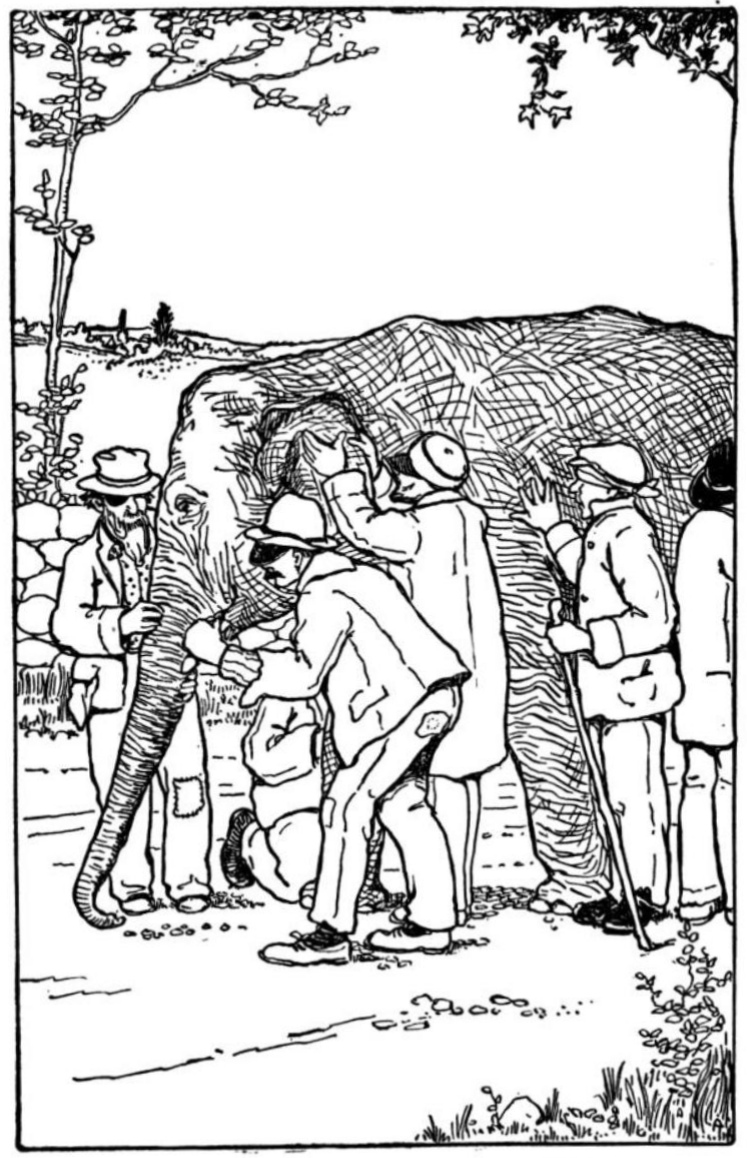
\includegraphics[width=0.4\textwidth]{images/Blind_men_and_elephant.jpg}
\end{center}

But unfortunately, threads have their own view of the world.

\end{frame}

\begin{frame}
  \frametitle{Reordering}

  
     Compilers and processors may reorder non-interfering memory
     operations.

      \[ T1: x = 1; r1 = y; \]

     If two statements are independent:
     \begin{itemize}
        \item OK to execute them in either order.
        \item (equivalently: publish their results to other threads).
     \end{itemize}

     Reordering is a major compiler tactic to produce speedup.
  
\end{frame}

%%%%%%%%%%%%%%%%%%%%%%%%%%%%%%%%%%%%%%%%%%%%%%%%%%%%%%%%%%%%%%%%%%%%%%%%%%%%%%%%

%%%%%%%%%%%%%%%%%%%%%%%%%%%%%%%%%%%%%%%%%%%%%%%%%%%%%%%%%%%%%%%%%%%%%%%%%%%%%%%%
\begin{frame}
  \frametitle{Memory Consistency Models}

Rust uses the same memory consistency models as \CPP.

It's the best attempt we have at modelling atomics because it is a very difficult subject

We need way of talking about the \alert{causality} of the program...


\end{frame}

\begin{frame}
\frametitle{Causality?}

\begin{center}
	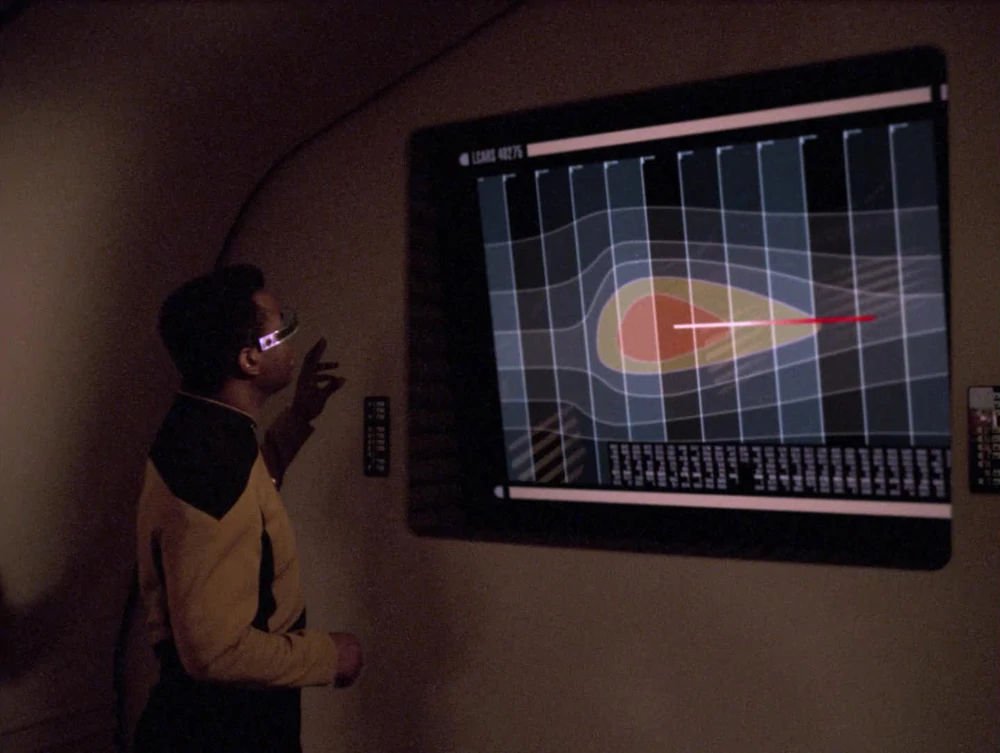
\includegraphics[width=0.7\textwidth]{images/causality-loop.png}
\end{center}



Establishing relationships between events such as ``event A happens before event B''. 
  
\end{frame}
%%%%%%%%%%%%%%%%%%%%%%%%%%%%%%%%%%%%%%%%%%%%%%%%%%%%%%%%%%%%%%%%%%%%%%%%%%%%%%%%


\begin{frame}
\frametitle{Our new Toolkit}

We can use a semaphore to ensure that one thing happens before another. 

The idea is the same, but our toolkit is a little bit different: it's the \alert{memory barrier} or
\alert{fence}. 

This type of barrier prevents reordering, or,
equivalently, ensures that memory operations become visible in the
right order.

\end{frame}




\begin{frame}
\frametitle{What have we got?}

The x86 architecture defines the following types of memory 
barriers:

\begin{itemize}
\item {\tt mfence}
\item {\tt sfence}
\item {\tt lfence}
\end{itemize}

\end{frame}


\begin{frame}[fragile]
\frametitle{Build Fences in the Right Place}

Consider the example again:
  \begin{lstlisting}[language=C]
                         f = 0

/* thread 1 */                     /* thread 2 */
while (f == 0) /* spin */;         x = 42;
// memory fence                    // memory fence
printf("%d", x);                   f = 1;
  \end{lstlisting}
This now prevents reordering, and we get the expected result.

Memory fences are costly in performance.

\end{frame}


\begin{frame}
\frametitle{Here Be Dragons}
The \CPP~standard includes a few other orderings that don't appear in this section because they aren't in Rust. 

But we'll cover Acquire-Release and Relaxed briefly. 

Neither comes with a recommendation to use it, but if you can prove that your use of it is correct, then you can do it. 

It may give a slight performance edge.


\end{frame}


\begin{frame}
\frametitle{Acquire and Release}

Acquire and Release make a good team! 

\begin{center}
	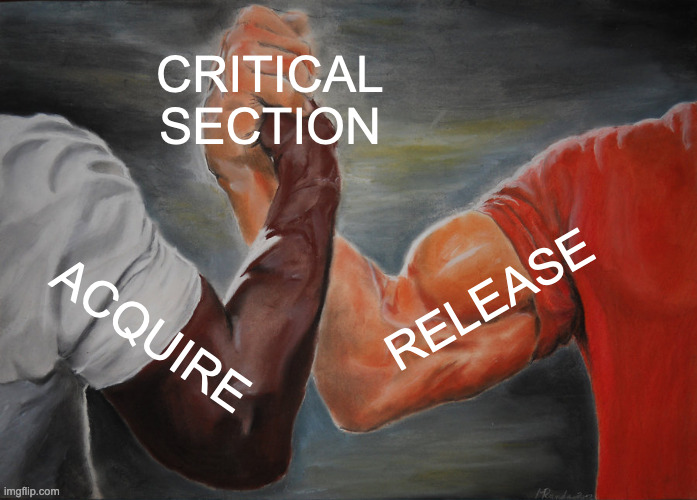
\includegraphics[width=0.4\textwidth]{images/acqrel.jpg}
\end{center}

By placing acquire at the start of a section and release after, anything in there is ``trapped'' and can't get out.

That makes them the perfect combination for a critical section.

\end{frame}


\begin{frame}[fragile]
\frametitle{Acquire/Release Spinlock}

\begin{lstlisting}[language=Rust]
use std::sync::Arc;
use std::sync::atomic::{AtomicBool, Ordering};
use std::thread;

fn main() {
    let lock = Arc::new(AtomicBool::new(false)); // value answers "am I locked?"

    // ... distribute lock to threads somehow ...

    // Try to acquire the lock by setting it to true
    while lock.compare_and_swap(false, true, Ordering::Acquire) { }
    // broke out of the loop, so we successfully acquired the lock!

    // ... scary data accesses ...

    // ok we're done, release the lock
    lock.store(false, Ordering::Release);
}
\end{lstlisting}


\end{frame}


\begin{frame}
\frametitle{Relaxed?}

Relaxed really does mean the compiler will take it easy, and all reorderings are possible.

A counter that simply adds and you aren't using the counter to synchronize any action.

\end{frame}


\begin{frame}
\frametitle{Matter, Order Does}

There have been a few reminders to use sequential consistency because atomics are hard to reason about and it's easy to get it wrong.

Consider an inconsistent state in a lock-free-queue structure...

We can actually look at the fix applied in the code.

\end{frame}


\end{document}

